\section{Evaluation}
\label{sec:evaluation}

\subsection{Protocol}
\label{sec:eval-protocol}

Every number in this section is produced by \texttt{make\_paper\_assets.py} from
\texttt{results/main.csv}; the manuscript does not contain a typed experimental
value. The matrix is $10$ seeds $\times$ $8$ scenarios $\times$ $10$ policies
$=800$ runs of $2{,}000$ epochs each, and all policies replay the same
observation and request stream for a given seed and scenario, so every
comparison is paired. \Cref{tab:params} lists the implementation parameters and
their values as read from the simulator.

For each policy we report six quantities. \emph{Invariant violations per
1{,}000 decisions} (IVR) counts granted requests whose action falls below the
I1/I2 floor; because I1 is an actuation envelope and I2 a safety envelope, this
metric is meaningful only for actuation and safety requests, and we report the
per-operation breakdown in \cref{tab:ivr-byop}. \emph{Malicious-grant rate}
counts malicious requests that were granted, whether or not the action satisfied
I1/I2; it is the residual exposure that survives the invariant layer.
\emph{False-denial rate} is the fraction of legitimate non-safety requests
denied. \emph{Safety-denial rate} is the fraction of safety-critical requests
denied. \emph{Mission utility} is the normalised net value from
\eqref{eq:utility} and \eqref{eq:score}, including energy and latency costs and,
for any granted action below the floor, the violation penalty $\rho=6.0$.
\emph{Calibration} is the Brier score and expected calibration error of the
belief each policy acts on. Unless stated otherwise, an ``attack mean'' is the
unweighted mean over the seven attack scenarios (DoS, downgrade, TEE, energy,
Byzantine, resonant, adaptive); the benign scenario is excluded from attack
aggregates because it contains no serious attack state.

Statistical comparisons aggregate each seed over the seven attack scenarios and
apply a two-sided Wilcoxon signed-rank test ($n=10$) against Full, with Holm
correction within each metric across the four baselines
(\cref{tab:stats}). With ten pairs the test is deliberately conservative; the smallest attainable
two-sided $p$-value is $0.00195$, so every $p_{\text{Holm}}=0.008$ in
\cref{tab:stats} is at the resolution floor and should be read as sign
consistency across seeds rather than as a precise significance level. We report
effect sizes next to $p$-values and do not treat a difference that fails to reach
the $0.05$ level as evidence of equivalence.

% Generated by make_paper_assets.py from simulator.py constants.
\begin{table}[t]
\centering
\small
\caption{Simulation and controller parameters. Values are read from the
implementation, not typed into the manuscript.}
\label{tab:params}
\resizebox{\textwidth}{!}{%
\begin{tabular}{lll}
\toprule
Group & Parameter & Value \\
\midrule
Deployment & nodes / seeds / epochs / policy runs & 24, 10, 2{,}000, 800 \\
Byzantine fraction & colluding nodes $f$ & 10/24 = 0.42 \\
Latent states & benign, recon, DoS, Byzantine, compromised & 5 \\
HMM persistence & $\operatorname{diag}(T)$ & 0.82 \\
Action lattice & $|\mathcal{A}|$ & 243 \\
Prior malice & $P_{\mathrm{malicious}}$ & 0.35 \\
Base detection & $p_{\mathrm{base}}$ & 0.05 \\
Auth detection & token / mutual / attest & 0.02, 0.18, 0.45 \\
IDS detection & off / header / deep & 0.00, 0.45, 0.70 \\
Rate-limit detection & off / 50 / 10 per s & 0.00, 0.15, 0.40 \\
Escalation & $\tau_{\mathrm{up}}$ & 0.60 \\
De-escalation & $\tau_{\mathrm{down}}$ & 0.30 \\
Conditional floor & $\tau_{\mathrm{risk}}$ & 0.55 \\
Strong floor & $\tau_{\mathrm{high}}$ & 0.90 \\
Dwell & epochs & 25 \\
Switch margin & $m$ & 0.06 \\
Trust midpoint / slope & $\tau_{\mathrm{TV}}$ / $s_{\mathrm{TV}}$ & 0.25 / 0.06 \\
Dispersion floor / span & $d_0$ / $d_1$ & 0.09 / 0.16 \\
Cost weights & $\lambda_E$ / $\lambda_L$ / $\gamma$ & 0.15 / 0.02 / 0.05 \\
Safety penalty & $\rho$ & 6.0 \\
\bottomrule
\end{tabular}}
\end{table}


\subsection{RQ1: Do hard invariants eliminate unsafe downgrades?}
\label{sec:rq1}

\Cref{tab:ivr} answers RQ1 directly. Every policy that enforces I1/I2 records
exactly $0.00$ invariant violations per $1{,}000$ decisions in all eight
scenarios. Static-High is zero because it always selects the strongest posture;
Static-Med is zero because it is a fixed mid-point that is raised to each
operation's structural floor; Threshold, Invariant-Only, Full$-$Hyst, Full$-$Cons,
Full and Oracle are zero because they install the node-side PEP re-check. The two policies that do not install
it violate the floor heavily: Static-Low at $393.31$ per $1{,}000$ and Risk-Only
at $327.41$, with attack-scenario values between $303.4$ and $403.9$. Risk-Only is
the informative case: it is a full Bayesian belief controller with the same
trust-weighted estimator as Full, it is granted the same belief stream, and it
still violates the floor at roughly the same rate as a policy that ignores risk
altogether, because nothing in its objective is non-negotiable. Adding the
invariant layer and the PEP re-check to that same estimator removes the
violations entirely.

The zero is structural, not statistical. \Cref{prop:structural} shows that a
granted actuation or safety request is either the constrained argmax, which lies
in $\Asafe$, or the I4 fallback $a_{\max}$, which also lies in $\Asafe$; the proof
makes no assumption about $b_t$. The experiment is a check on the implementation
of that argument, not a measurement of how often the estimator happens to be
right. The strongest empirical support is the \texttt{tee} scenario: Full's
belief is badly wrong there (Brier $0.437$), its utility drops to $0.058$---the
lowest of any attack scenario---and its malicious-grant rate rises to $0.473$---yet
its IVR stays at zero, because the belief can only remove actions from the
admissible set, not add them.

Two baselines also achieve zero IVR, and it is worth being explicit about why
this does not make the invariant layer redundant. Static-High never leaves the
strongest posture, and Static-Med is raised to the floor for each operation;
neither adapts. Threshold is zero only
because we implemented it with the same structural floor
(\texttt{STRUCT\_FLOOR}) rather than as a naive point-estimate threshold; without
that floor it would inherit the violation behaviour of Risk-Only, since it selects
actions from the unconstrained lattice when the score is below threshold. The
contribution of RQ1 is therefore not ``zero IVR'' in isolation but zero IVR
\emph{while adapting}, with the belief free to be wrong.

\Cref{tab:ivr-byop} makes the scope of the claim explicit. Read and write have no
structural floor by design, so their IVR is zero for every policy and says
nothing about posture strength; the guarantee constrains actuation and safety
traffic. On those classes the unconstrained baselines violate almost every
decision in an attack window ($979.81$ actuation and $996.76$ safety per
$1{,}000$ for Static-Low; $778.00$ and $996.76$ for Risk-Only), while every
PEP-enforcing policy records zero.

\begin{figure}[t]
\centering
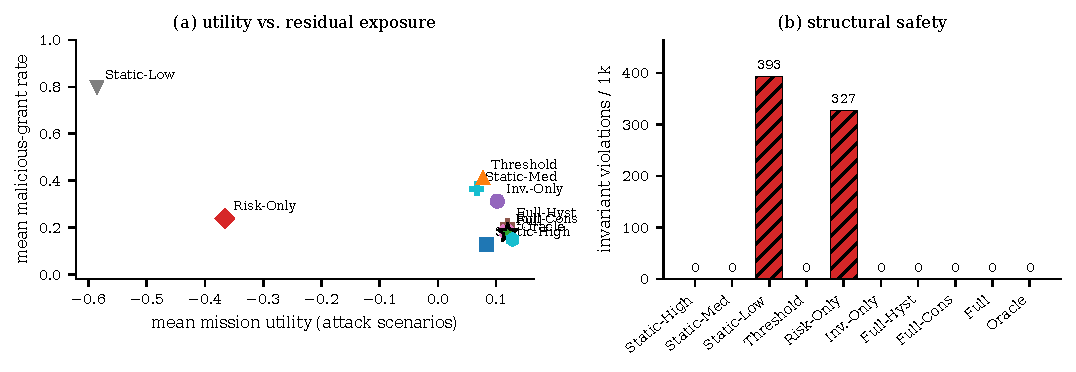
\includegraphics[width=\linewidth]{figures/fig_tradeoff.pdf}
\caption{(a) Mean attack-scenario utility against mean malicious-grant rate;
right and down is better. (b) Invariant violations per $1{,}000$ decisions.
Bars at zero are policies that install the PEP re-check; the two nonzero,
hatched bars are the unconstrained baselines. Static-High is safe and cheap in exposure
but sits at low utility and high false denial; Full keeps zero violations at
higher utility, at the cost of residual exposure concentrated in the
out-of-model TEE scenario.}
\label{fig:tradeoff}
\end{figure}

% Generated by make_paper_assets.py — do not edit by hand; regenerate.
\begin{table*}[t]
\centering
\scriptsize
\setlength{\tabcolsep}{3.0pt}
\caption{Invariant violations per 1,000 decisions (mean $\pm$ std over 10 seeds). A violation is a granted request whose action falls below the I1/I2 floor; zero is the design target and is achieved by every policy that enforces the unconditional invariants.}
\label{tab:ivr}
\resizebox{\textwidth}{!}{%
\begin{tabular}{lccccccccc}
\toprule
Policy & None & DoS & Down. & TEE & Energy & Byz. & Reson. & Adapt. & Attack mean \\
\midrule
Static-High & 0.00\,$\pm$\,0.00 & 0.00\,$\pm$\,0.00 & 0.00\,$\pm$\,0.00 & 0.00\,$\pm$\,0.00 & 0.00\,$\pm$\,0.00 & 0.00\,$\pm$\,0.00 & 0.00\,$\pm$\,0.00 & 0.00\,$\pm$\,0.00 & 0.00 \\
Static-Med & 0.00\,$\pm$\,0.00 & 0.00\,$\pm$\,0.00 & 0.00\,$\pm$\,0.00 & 0.00\,$\pm$\,0.00 & 0.00\,$\pm$\,0.00 & 0.00\,$\pm$\,0.00 & 0.00\,$\pm$\,0.00 & 0.00\,$\pm$\,0.00 & 0.00 \\
Static-Low & 352.74\,$\pm$\,7.01 & 402.54\,$\pm$\,12.16 & 402.85\,$\pm$\,9.76 & 398.36\,$\pm$\,8.86 & 347.03\,$\pm$\,6.62 & 396.10\,$\pm$\,6.47 & 402.40\,$\pm$\,12.26 & 403.87\,$\pm$\,9.81 & 393.31 \\
Threshold & 0.00\,$\pm$\,0.00 & 0.00\,$\pm$\,0.00 & 0.00\,$\pm$\,0.00 & 0.00\,$\pm$\,0.00 & 0.00\,$\pm$\,0.00 & 0.00\,$\pm$\,0.00 & 0.00\,$\pm$\,0.00 & 0.00\,$\pm$\,0.00 & 0.00 \\
Risk-Only & 352.05\,$\pm$\,7.04 & 309.44\,$\pm$\,8.71 & 309.41\,$\pm$\,9.88 & 391.52\,$\pm$\,8.33 & 342.75\,$\pm$\,6.71 & 326.41\,$\pm$\,6.38 & 303.36\,$\pm$\,5.21 & 308.98\,$\pm$\,5.76 & 327.41 \\
Inv.-Only & 0.00\,$\pm$\,0.00 & 0.00\,$\pm$\,0.00 & 0.00\,$\pm$\,0.00 & 0.00\,$\pm$\,0.00 & 0.00\,$\pm$\,0.00 & 0.00\,$\pm$\,0.00 & 0.00\,$\pm$\,0.00 & 0.00\,$\pm$\,0.00 & 0.00 \\
Full$-$Hyst & 0.00\,$\pm$\,0.00 & 0.00\,$\pm$\,0.00 & 0.00\,$\pm$\,0.00 & 0.00\,$\pm$\,0.00 & 0.00\,$\pm$\,0.00 & 0.00\,$\pm$\,0.00 & 0.00\,$\pm$\,0.00 & 0.00\,$\pm$\,0.00 & 0.00 \\
Full$-$Cons & 0.00\,$\pm$\,0.00 & 0.00\,$\pm$\,0.00 & 0.00\,$\pm$\,0.00 & 0.00\,$\pm$\,0.00 & 0.00\,$\pm$\,0.00 & 0.00\,$\pm$\,0.00 & 0.00\,$\pm$\,0.00 & 0.00\,$\pm$\,0.00 & 0.00 \\
\textbf{Full} & 0.00\,$\pm$\,0.00 & 0.00\,$\pm$\,0.00 & 0.00\,$\pm$\,0.00 & 0.00\,$\pm$\,0.00 & 0.00\,$\pm$\,0.00 & 0.00\,$\pm$\,0.00 & 0.00\,$\pm$\,0.00 & 0.00\,$\pm$\,0.00 & 0.00 \\
\emph{Oracle} & 0.00\,$\pm$\,0.00 & 0.00\,$\pm$\,0.00 & 0.00\,$\pm$\,0.00 & 0.00\,$\pm$\,0.00 & 0.00\,$\pm$\,0.00 & 0.00\,$\pm$\,0.00 & 0.00\,$\pm$\,0.00 & 0.00\,$\pm$\,0.00 & 0.00 \\
\bottomrule
\end{tabular}}
\end{table*}

% Generated by make_paper_assets.py — do not edit by hand; regenerate.
\begin{table}[t]
\centering
\scriptsize
\setlength{\tabcolsep}{3.5pt}
\caption{Invariant violations per 1{,}000 decisions by operation class
(attack-scenario mean over 10 seeds). I1 is an actuation envelope and I2 a
safety envelope, so read and write have no structural floor: a zero there
means the invariant does not constrain that class, not that the action was
strong. The unconstrained baselines violate the actuation and safety floors;
every policy that installs the PEP records zero.}
\label{tab:ivr-byop}
\resizebox{\textwidth}{!}{%
\begin{tabular}{lccc}
\toprule
Policy & read + write & actuate & safety \\
\midrule
Static-Low & 0.00 & 979.81 & 996.76 \\
Risk-Only & 0.00 & 778.00 & 996.76 \\
Threshold & 0.00 & 0.00 & 0.00 \\
Inv.-Only & 0.00 & 0.00 & 0.00 \\
\textbf{Full} & 0.00 & 0.00 & 0.00 \\
\bottomrule
\end{tabular}}
\end{table}


\subsection{RQ2: What is the utility cost of the guarantee?}
\label{sec:rq2}

\Cref{tab:utility,tab:falsedeny,tab:exposure} give the three sides of the
trade-off: mission utility, false denial, and residual malicious grants.
\Cref{fig:tradeoff}(a) plots the first against the third.

\paragraph{Utility.} Full attains $0.120$ mean attack-scenario utility, against
$0.084$ for Static-High, $0.077$ for Threshold, $0.102$ for Invariant-Only and
$-0.366$ for Risk-Only. The paired difference against Static-High is $+0.036$
($p_{\text{Holm}}=0.008$) and against Threshold $+0.043$
($p_{\text{Holm}}=0.008$); against Risk-Only and Static-Low the difference is
$+0.486$ and $+0.706$ respectively (\cref{tab:stats}). The absolute gain over
Static-High is modest, which is the honest reading: a safety floor does not
create value, it prevents a particular kind of loss. The larger gains are against
policies that either deny legitimate traffic or fail to detect malicious traffic.

Full is within $0.005$ of the best non-oracle utility in every attack scenario.
The scenario breakdown is more informative than the mean. Full's advantage over
Static-High is largest under energy inflation ($0.174$ versus $0.122$), and it
also gains under the adaptive attacker ($0.127$ versus $0.089$) and the Byzantine
minority ($0.097$ versus $0.057$), where the trust-weighted belief separates
colluding from honest nodes and tracks slow drift. It is close to the oracle under
DoS ($0.131$ versus $0.132$) and energy inflation ($0.174$ versus $0.186$). It
does not lose to Static-High in the \texttt{tee} scenario ($0.058$ versus
$0.053$), but that comparison is misleading: a spoofed anchor makes both postures
select cheap admissible actions, and the cost appears in residual exposure rather
than in utility. The in-model
downgrade no longer produces a utility loss: Full reaches $0.129$ against $0.090$
for Static-High, because the anchor and dispersion keep the belief calibrated.

\paragraph{False denial.} Full denies $0.027$ of legitimate requests over the
attack scenarios, compared with $0.088$ for Static-High, $0.019$ for Threshold,
and $0.003$ for Static-Low. The low Static-Low number is not an achievement: it
grants almost everything, including $0.798$ of malicious requests. Against
Static-High the reduction in false denial is a factor of three, and it is the
main source of Full's utility advantage. Threshold is slightly better than Full on
this metric but pays for it with a $2.3\times$ higher malicious-grant rate
($0.414$).

\paragraph{Residual exposure.} This is where the design is weakest. Full grants
$0.177$ of malicious requests over the attack scenarios, against $0.127$ for
Static-High, $0.148$ for Oracle, $0.312$ for Invariant-Only, $0.414$ for Threshold
and $0.798$ for Static-Low. Static-High is better because it always buys the
deepest inspection and the strongest authentication; Full buys them only when the
belief or I3 says they are needed. The paired difference of $+0.050$ malicious
grants against Static-High is significant ($p_{\text{Holm}}=0.008$) and goes the
wrong way.

The per-scenario decomposition matters for interpreting that gap. Of the $0.050$,
$0.030$ comes from the single out-of-model \texttt{tee} scenario, where Full
grants $0.473$ against Static-High's $0.265$. Excluding \texttt{tee}, Full is
$0.128$ against $0.104$. The remaining in-model gap is small and concentrated
under Byzantine attack ($0.293$ versus $0.253$), where a colluding minority that
keeps every modality plausible is genuinely hard to separate from honest
neighbours. Under DoS, downgrade, resonant and adaptive attack Full is within
$0.03$ of Static-High. The invariant layer bounds the \emph{worst action} but not
the \emph{detection probability} of that action: an attacker who holds a valid
credential and spoofs a benign context can be granted a request that satisfies I1
and still be malicious. This is a real limitation of a decision-layer
contribution, and we state it as such rather than presenting utility alone.

\begin{figure}[t]
\centering
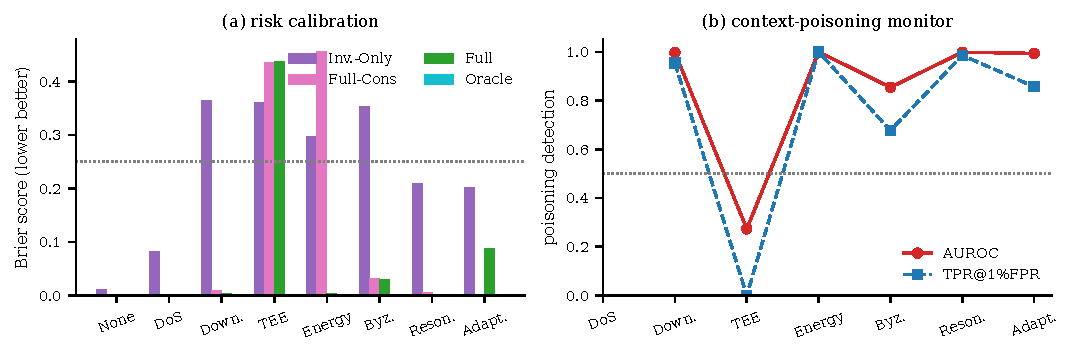
\includegraphics[width=\linewidth]{figures/fig_calibration.pdf}
\caption{(a) Brier score of the risk estimate by scenario for four policies.
(b) Poisoning detection: AUROC and TPR at $1\,\%$ FPR for the consistency
monitor. The \texttt{tee} scenario is the honest negative result: a spoofed
attestation anchor drives both the belief and the monitor below chance. The
in-model downgrade, by contrast, is detected.}
\label{fig:calibration}
\end{figure}

% Generated by make_paper_assets.py — do not edit by hand; regenerate.
\begin{table*}[t]
\centering
\scriptsize
\setlength{\tabcolsep}{3.0pt}
\caption{Mission utility (mean $\pm$ std over 10 seeds; higher is better). Utility normalises value, damage, denial cost, energy and latency by $V_{\max}$; it is negative when denials and damage dominate. Bold marks the best non-oracle policy per scenario.}
\label{tab:utility}
\resizebox{\textwidth}{!}{%
\begin{tabular}{lccccccccc}
\toprule
Policy & None & DoS & Down. & TEE & Energy & Byz. & Reson. & Adapt. & Attack mean \\
\midrule
Static-High & 0.121\,$\pm$\,0.004 & 0.090\,$\pm$\,0.007 & 0.090\,$\pm$\,0.007 & 0.053\,$\pm$\,0.012 & 0.122\,$\pm$\,0.006 & 0.057\,$\pm$\,0.008 & 0.087\,$\pm$\,0.004 & 0.089\,$\pm$\,0.004 & 0.084 \\
Static-Med & 0.162\,$\pm$\,0.003 & 0.064\,$\pm$\,0.015 & 0.065\,$\pm$\,0.013 & 0.025\,$\pm$\,0.017 & 0.162\,$\pm$\,0.004 & 0.033\,$\pm$\,0.016 & 0.057\,$\pm$\,0.009 & 0.062\,$\pm$\,0.011 & 0.067 \\
Static-Low & -0.330\,$\pm$\,0.009 & -0.629\,$\pm$\,0.035 & -0.632\,$\pm$\,0.024 & -0.620\,$\pm$\,0.034 & -0.322\,$\pm$\,0.007 & -0.608\,$\pm$\,0.031 & -0.648\,$\pm$\,0.038 & -0.640\,$\pm$\,0.033 & -0.586 \\
Threshold & 0.183\,$\pm$\,0.003 & 0.108\,$\pm$\,0.010 & 0.060\,$\pm$\,0.016 & 0.028\,$\pm$\,0.018 & 0.155\,$\pm$\,0.006 & 0.039\,$\pm$\,0.017 & 0.084\,$\pm$\,0.009 & 0.068\,$\pm$\,0.012 & 0.077 \\
Risk-Only & -0.331\,$\pm$\,0.009 & -0.316\,$\pm$\,0.012 & -0.318\,$\pm$\,0.010 & -0.599\,$\pm$\,0.036 & -0.323\,$\pm$\,0.007 & -0.376\,$\pm$\,0.012 & -0.313\,$\pm$\,0.009 & -0.319\,$\pm$\,0.008 & -0.366 \\
Inv.-Only & 0.179\,$\pm$\,0.003 & 0.121\,$\pm$\,0.009 & 0.090\,$\pm$\,0.014 & \textbf{0.059\,$\pm$\,0.023} & 0.167\,$\pm$\,0.005 & 0.048\,$\pm$\,0.017 & 0.115\,$\pm$\,0.006 & 0.115\,$\pm$\,0.008 & 0.102 \\
Full$-$Hyst & \textbf{0.184\,$\pm$\,0.003} & \textbf{0.135\,$\pm$\,0.006} & \textbf{0.133\,$\pm$\,0.008} & 0.030\,$\pm$\,0.018 & \textbf{0.179\,$\pm$\,0.004} & \textbf{0.100\,$\pm$\,0.011} & \textbf{0.128\,$\pm$\,0.005} & \textbf{0.132\,$\pm$\,0.005} & 0.119 \\
Full$-$Cons & 0.179\,$\pm$\,0.003 & 0.131\,$\pm$\,0.006 & 0.127\,$\pm$\,0.008 & 0.053\,$\pm$\,0.021 & 0.166\,$\pm$\,0.005 & 0.097\,$\pm$\,0.010 & 0.124\,$\pm$\,0.004 & 0.128\,$\pm$\,0.005 & 0.118 \\
\textbf{Full} & 0.177\,$\pm$\,0.003 & 0.131\,$\pm$\,0.006 & 0.129\,$\pm$\,0.008 & 0.058\,$\pm$\,0.014 & 0.174\,$\pm$\,0.004 & 0.097\,$\pm$\,0.010 & 0.124\,$\pm$\,0.004 & 0.127\,$\pm$\,0.005 & 0.120 \\
\emph{Oracle} & 0.182\,$\pm$\,0.003 & 0.132\,$\pm$\,0.007 & 0.130\,$\pm$\,0.008 & 0.093\,$\pm$\,0.011 & 0.186\,$\pm$\,0.004 & 0.100\,$\pm$\,0.010 & 0.126\,$\pm$\,0.004 & 0.130\,$\pm$\,0.005 & 0.128 \\
\bottomrule
\end{tabular}}
\end{table*}

% Generated by make_paper_assets.py — do not edit by hand; regenerate.
\begin{table*}[t]
\centering
\scriptsize
\setlength{\tabcolsep}{3.0pt}
\caption{False-denial rate on legitimate requests (mean $\pm$ std over 10 seeds; lower is better). Bold marks the best non-oracle policy per scenario.}
\label{tab:falsedeny}
\resizebox{\textwidth}{!}{%
\begin{tabular}{lccccccccc}
\toprule
Policy & None & DoS & Down. & TEE & Energy & Byz. & Reson. & Adapt. & Attack mean \\
\midrule
Static-High & 0.087\,$\pm$\,0.004 & 0.090\,$\pm$\,0.004 & 0.089\,$\pm$\,0.004 & 0.087\,$\pm$\,0.009 & 0.089\,$\pm$\,0.003 & 0.089\,$\pm$\,0.005 & 0.086\,$\pm$\,0.004 & 0.085\,$\pm$\,0.005 & 0.088 \\
Static-Med & 0.024\,$\pm$\,0.002 & 0.026\,$\pm$\,0.002 & 0.024\,$\pm$\,0.003 & 0.024\,$\pm$\,0.004 & 0.025\,$\pm$\,0.002 & 0.025\,$\pm$\,0.002 & 0.024\,$\pm$\,0.003 & 0.024\,$\pm$\,0.003 & 0.024 \\
Static-Low & \textbf{0.003\,$\pm$\,0.000} & \textbf{0.003\,$\pm$\,0.001} & \textbf{0.003\,$\pm$\,0.001} & \textbf{0.003\,$\pm$\,0.001} & \textbf{0.003\,$\pm$\,0.001} & \textbf{0.003\,$\pm$\,0.001} & \textbf{0.003\,$\pm$\,0.001} & \textbf{0.003\,$\pm$\,0.001} & 0.003 \\
Threshold & 0.007\,$\pm$\,0.001 & 0.030\,$\pm$\,0.002 & 0.008\,$\pm$\,0.002 & 0.008\,$\pm$\,0.002 & 0.044\,$\pm$\,0.004 & 0.008\,$\pm$\,0.002 & 0.024\,$\pm$\,0.003 & 0.012\,$\pm$\,0.002 & 0.019 \\
Risk-Only & 0.003\,$\pm$\,0.001 & 0.017\,$\pm$\,0.002 & 0.016\,$\pm$\,0.003 & 0.004\,$\pm$\,0.001 & 0.010\,$\pm$\,0.002 & 0.013\,$\pm$\,0.001 & 0.017\,$\pm$\,0.003 & 0.015\,$\pm$\,0.003 & 0.013 \\
Inv.-Only & 0.015\,$\pm$\,0.003 & 0.030\,$\pm$\,0.003 & 0.013\,$\pm$\,0.004 & 0.014\,$\pm$\,0.002 & 0.030\,$\pm$\,0.004 & 0.011\,$\pm$\,0.002 & 0.027\,$\pm$\,0.003 & 0.017\,$\pm$\,0.002 & 0.020 \\
Full$-$Hyst & 0.012\,$\pm$\,0.003 & 0.027\,$\pm$\,0.002 & 0.024\,$\pm$\,0.003 & 0.011\,$\pm$\,0.003 & 0.017\,$\pm$\,0.003 & 0.028\,$\pm$\,0.004 & 0.026\,$\pm$\,0.003 & 0.024\,$\pm$\,0.003 & 0.022 \\
Full$-$Cons & 0.018\,$\pm$\,0.004 & 0.032\,$\pm$\,0.003 & 0.027\,$\pm$\,0.003 & 0.015\,$\pm$\,0.003 & 0.032\,$\pm$\,0.003 & 0.026\,$\pm$\,0.002 & 0.029\,$\pm$\,0.003 & 0.028\,$\pm$\,0.003 & 0.027 \\
\textbf{Full} & 0.020\,$\pm$\,0.004 & 0.032\,$\pm$\,0.003 & 0.029\,$\pm$\,0.003 & 0.018\,$\pm$\,0.004 & 0.023\,$\pm$\,0.003 & 0.026\,$\pm$\,0.002 & 0.031\,$\pm$\,0.003 & 0.029\,$\pm$\,0.004 & 0.027 \\
\emph{Oracle} & 0.013\,$\pm$\,0.002 & 0.031\,$\pm$\,0.004 & 0.029\,$\pm$\,0.003 & 0.026\,$\pm$\,0.004 & 0.008\,$\pm$\,0.001 & 0.025\,$\pm$\,0.003 & 0.029\,$\pm$\,0.002 & 0.026\,$\pm$\,0.003 & 0.025 \\
\bottomrule
\end{tabular}}
\end{table*}

% Generated by make_paper_assets.py — do not edit by hand; regenerate.
\begin{table*}[t]
\centering
\scriptsize
\setlength{\tabcolsep}{3.0pt}
\caption{Residual exposure: fraction of malicious requests granted (mean $\pm$ std over 10 seeds; lower is better). This is not an invariant violation: the action may still satisfy I1/I2, but a credential-holding attacker was not detected. Bold marks the best non-oracle policy per scenario.}
\label{tab:exposure}
\resizebox{\textwidth}{!}{%
\begin{tabular}{lccccccccc}
\toprule
Policy & None & DoS & Down. & TEE & Energy & Byz. & Reson. & Adapt. & Attack mean \\
\midrule
Static-High & \textbf{0.000\,$\pm$\,0.000} & \textbf{0.088\,$\pm$\,0.014} & \textbf{0.091\,$\pm$\,0.011} & \textbf{0.265\,$\pm$\,0.023} & \textbf{0.000\,$\pm$\,0.000} & \textbf{0.253\,$\pm$\,0.021} & \textbf{0.094\,$\pm$\,0.012} & \textbf{0.095\,$\pm$\,0.010} & 0.127 \\
Static-Med & 0.000\,$\pm$\,0.000 & 0.367\,$\pm$\,0.034 & 0.357\,$\pm$\,0.020 & 0.554\,$\pm$\,0.021 & 0.000\,$\pm$\,0.000 & 0.541\,$\pm$\,0.017 & 0.364\,$\pm$\,0.023 & 0.370\,$\pm$\,0.016 & 0.365 \\
Static-Low & 0.000\,$\pm$\,0.000 & 0.931\,$\pm$\,0.011 & 0.931\,$\pm$\,0.007 & 0.928\,$\pm$\,0.012 & 0.000\,$\pm$\,0.000 & 0.938\,$\pm$\,0.010 & 0.926\,$\pm$\,0.012 & 0.932\,$\pm$\,0.014 & 0.798 \\
Threshold & 0.000\,$\pm$\,0.000 & 0.178\,$\pm$\,0.019 & 0.573\,$\pm$\,0.024 & 0.695\,$\pm$\,0.019 & 0.000\,$\pm$\,0.000 & 0.687\,$\pm$\,0.016 & 0.335\,$\pm$\,0.016 & 0.430\,$\pm$\,0.019 & 0.414 \\
Risk-Only & 0.000\,$\pm$\,0.000 & 0.111\,$\pm$\,0.013 & 0.122\,$\pm$\,0.013 & 0.885\,$\pm$\,0.047 & 0.000\,$\pm$\,0.000 & 0.302\,$\pm$\,0.019 & 0.119\,$\pm$\,0.013 & 0.125\,$\pm$\,0.013 & 0.238 \\
Inv.-Only & 0.000\,$\pm$\,0.000 & 0.182\,$\pm$\,0.018 & 0.382\,$\pm$\,0.051 & 0.545\,$\pm$\,0.077 & 0.000\,$\pm$\,0.000 & 0.631\,$\pm$\,0.030 & 0.196\,$\pm$\,0.015 & 0.249\,$\pm$\,0.017 & 0.312 \\
Full$-$Hyst & 0.000\,$\pm$\,0.000 & 0.110\,$\pm$\,0.013 & 0.121\,$\pm$\,0.014 & 0.695\,$\pm$\,0.019 & 0.000\,$\pm$\,0.000 & 0.299\,$\pm$\,0.018 & 0.119\,$\pm$\,0.013 & 0.123\,$\pm$\,0.012 & 0.209 \\
Full$-$Cons & 0.000\,$\pm$\,0.000 & 0.110\,$\pm$\,0.013 & 0.139\,$\pm$\,0.012 & 0.493\,$\pm$\,0.072 & 0.000\,$\pm$\,0.000 & 0.294\,$\pm$\,0.019 & 0.127\,$\pm$\,0.017 & 0.122\,$\pm$\,0.013 & 0.184 \\
\textbf{Full} & 0.000\,$\pm$\,0.000 & 0.111\,$\pm$\,0.013 & 0.120\,$\pm$\,0.015 & 0.473\,$\pm$\,0.063 & 0.000\,$\pm$\,0.000 & 0.293\,$\pm$\,0.019 & 0.119\,$\pm$\,0.013 & 0.123\,$\pm$\,0.012 & 0.177 \\
\emph{Oracle} & 0.000\,$\pm$\,0.000 & 0.110\,$\pm$\,0.013 & 0.113\,$\pm$\,0.012 & 0.296\,$\pm$\,0.022 & 0.000\,$\pm$\,0.000 & 0.285\,$\pm$\,0.020 & 0.116\,$\pm$\,0.015 & 0.118\,$\pm$\,0.010 & 0.148 \\
\bottomrule
\end{tabular}}
\end{table*}

% Generated by make_paper_assets.py. Paired by seed; values are means over the
% seven attack scenarios per seed (n=10). Wilcoxon signed-rank, Holm within metric.
\begin{table}[t]
\centering
\small
\caption{Paired comparison against Full, aggregated over the seven attack scenarios
per seed ($n=10$). $\Delta$ is Full minus baseline; a negative $\Delta$ for
malicious grant and IVR is better. $p_{\text{Holm}}$ is within the metric across
the four baselines. Em dashes mark identical vectors (no test).}
\label{tab:stats}
\begin{tabular}{lcccccc}
\toprule
 & \multicolumn{2}{c}{Utility $\uparrow$} & \multicolumn{2}{c}{Malicious grant $\downarrow$} & \multicolumn{2}{c}{IVR/1k $\downarrow$} \\
\cmidrule(lr){2-3}\cmidrule(lr){4-5}\cmidrule(lr){6-7}
Baseline & $\Delta$ & $p_{\text{Holm}}$ & $\Delta$ & $p_{\text{Holm}}$ & $\Delta$ & $p_{\text{Holm}}$ \\
\midrule
Static-High & +0.036 & 0.008 & +0.050 & 0.008 & 0.000 & -- \\
Threshold & +0.043 & 0.008 & -0.237 & 0.008 & 0.000 & -- \\
Risk-Only & +0.486 & 0.008 & -0.061 & 0.008 & -327.409 & 0.004 \\
Static-Low & +0.706 & 0.008 & -0.621 & 0.008 & -393.308 & 0.004 \\
\bottomrule
\end{tabular}
\end{table}


\subsection{RQ3: Is the belief calibrated under poisoning?}
\label{sec:rq3}

\Cref{tab:calibration,tab:detection} and \cref{fig:calibration} answer RQ3.
The answer is conditional on what the adversary can spoof.

\paragraph{Calibration.} Full's Brier score is $0.002$ under benign operation,
$0.002$ under DoS, $0.003$ under in-model downgrade, $0.003$ under energy
inflation, $0.030$ under Byzantine attack and $0.088$ under the adaptive attacker.
Those are close to the oracle's zero and far below the $0.25$ of an uninformative
forecast. The single failure is the out-of-model \texttt{tee} scenario ($0.437$),
where the anchor itself is moved toward benign and the belief becomes confidently
wrong. The contrast with the earlier intuition is important: a downgrade that
leaves the attested device modality and the cross-node dispersion intact is
\emph{not} a belief failure, because those two signals still carry the attack.

\paragraph{The value of trust weighting.} The ablation isolates the fusion
mechanism. Full$-$Cons uses uniform modality weights and is otherwise identical.
Its Brier score under energy inflation is $0.455$ against $0.003$ for Full, a
factor of about $140$, and $0.436$ under \texttt{tee} against $0.437$---the trust
weighting cannot rescue a scenario in which the adversary moves every modality
coherently, but it almost eliminates the damage when only the network and
security modalities are inflated. Invariant-Only, which replaces the belief with a
point anomaly score, has Brier $0.296$ under energy inflation and $0.354$ under
Byzantine attack; the continuous belief with trust weights is substantially better
in both. The advantage is not uniform: under the adaptive attacker Full$-$Cons is
better calibrated ($0.003$ versus $0.088$), because its conservatism lowers
confidence when the attack is slow. Trust weighting buys robustness to partial
poisoning, not uniformly lower Brier.

\paragraph{Detection.} The consistency monitor detects energy inflation almost
perfectly (AUROC $1.000$, TPR@$1\,\%$FPR $1.000$), resonant pulsing well
($0.999$, $0.986$), the adaptive attacker well ($0.994$, $0.857$), the in-model
downgrade well ($0.997$, $0.954$) and the Byzantine minority moderately
($0.854$, $0.677$). The \texttt{tee} scenario is below chance (AUROC $0.273$,
TPR $0.000$): when the adversary controls every modality including the anchor,
the consistency score is \emph{lower} during the attack than during benign
operation, so a monitor that thresholds disagreement is systematically fooled.
The belief AUROC in that scenario is $0.210$, also below chance.

This result is not a bug to be tuned away; it is the reason the architecture
separates the estimator from the guarantee. If the safety argument depended on
the belief being right, an anchor compromise would be a safety failure. Because I1
and I2 are unconditional, the same scenario produces zero invariant violations and
a bounded (if unsatisfactory) posture. The correct response to
\cref{tab:detection} is to strengthen the unconditional floor, not to add
confidence to a monitor that cannot see the attack; \cref{sec:rq5-floor}
quantifies that trade.

% Generated by make_paper_assets.py — do not edit by hand; regenerate.
\begin{table*}[t]
\centering
\scriptsize
\setlength{\tabcolsep}{3.5pt}
\caption{Calibration of the risk estimate each policy acts on: Brier score and
expected calibration error (mean over 10 seeds; lower is better). Static and
threshold policies have no risk estimate, so they are omitted. Risk-Only and
Full share the same trust-weighted belief, so their calibration rows coincide;
they differ in the admissible set and the PEP re-check.}
\label{tab:calibration}
\resizebox{\textwidth}{!}{%
\begin{tabular}{llcccccccc}
\toprule
Metric & Policy & None & DoS & Down. & TEE & Energy & Byz. & Reson. & Adapt. \\
\midrule
Brier & Risk-Only & 0.002\,$\pm$\,0.001 & 0.002\,$\pm$\,0.000 & 0.003\,$\pm$\,0.001 & 0.437\,$\pm$\,0.041 & 0.003\,$\pm$\,0.001 & 0.030\,$\pm$\,0.006 & 0.002\,$\pm$\,0.001 & 0.088\,$\pm$\,0.024 \\
 & Inv.-Only & 0.010\,$\pm$\,0.000 & 0.082\,$\pm$\,0.006 & 0.364\,$\pm$\,0.021 & 0.360\,$\pm$\,0.033 & 0.296\,$\pm$\,0.029 & 0.354\,$\pm$\,0.036 & 0.209\,$\pm$\,0.014 & 0.202\,$\pm$\,0.020 \\
 & Full$-$Cons & 0.001\,$\pm$\,0.000 & 0.000\,$\pm$\,0.000 & 0.008\,$\pm$\,0.001 & 0.436\,$\pm$\,0.041 & 0.455\,$\pm$\,0.046 & 0.031\,$\pm$\,0.006 & 0.005\,$\pm$\,0.002 & 0.003\,$\pm$\,0.003 \\
 & \textbf{Full} & 0.002\,$\pm$\,0.001 & 0.002\,$\pm$\,0.000 & 0.003\,$\pm$\,0.001 & 0.437\,$\pm$\,0.041 & 0.003\,$\pm$\,0.001 & 0.030\,$\pm$\,0.006 & 0.002\,$\pm$\,0.001 & 0.088\,$\pm$\,0.024 \\
 & \emph{Oracle} & 0.000\,$\pm$\,0.000 & 0.000\,$\pm$\,0.000 & 0.000\,$\pm$\,0.000 & 0.000\,$\pm$\,0.000 & 0.000\,$\pm$\,0.000 & 0.000\,$\pm$\,0.000 & 0.000\,$\pm$\,0.000 & 0.000\,$\pm$\,0.000 \\
\midrule
ECE & Risk-Only & 0.010\,$\pm$\,0.001 & 0.006\,$\pm$\,0.001 & 0.006\,$\pm$\,0.001 & 0.435\,$\pm$\,0.041 & 0.015\,$\pm$\,0.002 & 0.043\,$\pm$\,0.008 & 0.006\,$\pm$\,0.001 & 0.117\,$\pm$\,0.028 \\
 & Inv.-Only & 0.078\,$\pm$\,0.001 & 0.205\,$\pm$\,0.012 & 0.371\,$\pm$\,0.026 & 0.360\,$\pm$\,0.039 & 0.405\,$\pm$\,0.034 & 0.339\,$\pm$\,0.043 & 0.235\,$\pm$\,0.021 & 0.310\,$\pm$\,0.022 \\
 & Full$-$Cons & 0.008\,$\pm$\,0.001 & 0.004\,$\pm$\,0.001 & 0.015\,$\pm$\,0.003 & 0.434\,$\pm$\,0.041 & 0.459\,$\pm$\,0.046 & 0.046\,$\pm$\,0.008 & 0.010\,$\pm$\,0.001 & 0.010\,$\pm$\,0.004 \\
 & \textbf{Full} & 0.010\,$\pm$\,0.001 & 0.006\,$\pm$\,0.001 & 0.006\,$\pm$\,0.001 & 0.435\,$\pm$\,0.041 & 0.015\,$\pm$\,0.002 & 0.043\,$\pm$\,0.008 & 0.006\,$\pm$\,0.001 & 0.117\,$\pm$\,0.028 \\
 & \emph{Oracle} & 0.000\,$\pm$\,0.000 & 0.000\,$\pm$\,0.000 & 0.000\,$\pm$\,0.000 & 0.000\,$\pm$\,0.000 & 0.000\,$\pm$\,0.000 & 0.000\,$\pm$\,0.000 & 0.000\,$\pm$\,0.000 & 0.000\,$\pm$\,0.000 \\
\bottomrule
\end{tabular}}
\end{table*}

% Generated by make_paper_assets.py — do not edit by hand; regenerate.
\begin{table}[t]
\centering
\small
\caption{Context-poisoning detection and belief discrimination by scenario
(mean over 10 seeds). Poison AUROC/TPR use the monitor's consistency score;
belief AUROC uses the Full policy's $P(\text{serious attack})$. Dashes mark
scenarios without poisoned epochs or without a serious-attack state.}
\label{tab:detection}
\begin{tabular}{lcccc}
\toprule
Scenario & Poison AUROC & TPR@1\%FPR & Belief AUROC & Brier (Full) \\
\midrule
None & -- & -- & -- & 0.002 \\
DoS & -- & -- & 1.000 & 0.002 \\
Down. & 0.997 & 0.954 & 1.000 & 0.003 \\
TEE & 0.273 & 0.000 & 0.210 & 0.437 \\
Energy & 1.000 & 1.000 & -- & 0.003 \\
Byz. & 0.854 & 0.677 & 0.997 & 0.030 \\
Reson. & 0.999 & 0.986 & 1.000 & 0.002 \\
Adapt. & 0.994 & 0.857 & 0.995 & 0.088 \\
\bottomrule
\end{tabular}
\end{table}


\subsection{RQ4: Does per-operation fail-safe semantics work?}
\label{sec:rq4}

\Cref{tab:safety} reports denial of safety-critical requests. Full denies
$0.029$ of them over the attack scenarios, against $0.088$ for Static-High and
$0.039$ for Threshold. Static-Low and Risk-Only deny only $0.003$, but they do so
by not enforcing I2: their safety-critical requests are served by weak actions
with low false-positive probability, which is exactly the failure I4 is designed
to prevent. Among policies that enforce I2, Full is tied for the lowest
safety-denial rate because it selects the cheapest action that satisfies the
envelope, rather than the maximal action.

The residual $0.029$ is not a policy denial. Deny is absent from the admissible
set for safety operations by I4, so every one of those denials is a stochastic
authentication or inspection false positive on an otherwise admissible action.
A caveat on scope: safety requests are legitimate in the simulator, so this
measures the mechanism false-positive floor, not an adversary deliberately
trying to suppress a safety action. Goal (ii) of the threat model is therefore
not separately instantiated; doing so would require forged or replayed safety
credentials and is left to future work.
This is the correct failure semantics: the controller does not choose to deny a
safety request, and the invariant layer does not permit it. The absolute level of
$0.029$ is a property of the I2 floor, not of adaptation: any policy that selects
an action at that floor inherits roughly the same mechanism false-positive rate.
What adaptation changes is which admissible action is selected---Full and
Invariant-Only take the cheapest, Threshold a stronger one, and Static-High a
stronger envelope still---so the comparison among floor-enforcing policies is
about the excess strength they buy, not about whether I2 is enforced. The exhaustive
test enumerates all $243$ actions for all four operation classes, checks that the
admissible set is non-empty for a $41$-point grid of $\attack\in[0,1]$, and
asserts that the conditional mask is a subset of the structural mask. A second
test exercises the empty-mask fallback and the PEP re-check, and a third runs
every adaptive policy on a live stream and finds no granted action outside I1/I2.
These tests verify the decision layer, not the cryptographic primitives; the
latter are assumed correct.

The comparison with a global fail-closed policy is implicit in Static-High's
$0.088$: a design that always uses the strongest envelope pays roughly three
times the safety-denial rate of one that selects the cheapest admissible action.
The comparison with a global fail-open policy is Static-Low's $0.003$ at the cost
of $393.31$ invariant violations per $1{,}000$ decisions. Neither global semantics
is acceptable; the per-operation envelope is what allows the controller to be
available for safety traffic without being permissive for actuation.

% Generated by make_paper_assets.py — do not edit by hand; regenerate.
\begin{table*}[t]
\centering
\scriptsize
\setlength{\tabcolsep}{3.5pt}
\caption{Denial rate on safety-critical requests (mean $\pm$ std over 10 seeds;
lower is better). Deny is inadmissible for this operation class (I4), so every
denial is a stochastic authentication/IDS false positive, not a policy choice.
The rate depends on which admissible action is selected inside the I2 floor,
which is why Threshold differs from the policies that select the cheapest one.}
\label{tab:safety}
\resizebox{\textwidth}{!}{%
\begin{tabular}{lccccccccc}
\toprule
Policy & None & DoS & Down. & TEE & Energy & Byz. & Reson. & Adapt. & Attack mean \\
\midrule
Static-High & 0.089\,$\pm$\,0.012 & 0.095\,$\pm$\,0.015 & 0.087\,$\pm$\,0.014 & 0.086\,$\pm$\,0.020 & 0.082\,$\pm$\,0.014 & 0.091\,$\pm$\,0.012 & 0.091\,$\pm$\,0.016 & 0.087\,$\pm$\,0.019 & 0.088 \\
Static-Med & 0.038\,$\pm$\,0.014 & 0.037\,$\pm$\,0.010 & 0.041\,$\pm$\,0.011 & 0.037\,$\pm$\,0.012 & 0.039\,$\pm$\,0.011 & 0.041\,$\pm$\,0.010 & 0.041\,$\pm$\,0.010 & 0.038\,$\pm$\,0.010 & 0.039 \\
Static-Low & 0.002\,$\pm$\,0.003 & 0.003\,$\pm$\,0.003 & 0.002\,$\pm$\,0.002 & 0.004\,$\pm$\,0.003 & 0.004\,$\pm$\,0.005 & 0.003\,$\pm$\,0.003 & 0.004\,$\pm$\,0.004 & 0.003\,$\pm$\,0.002 & 0.003 \\
Threshold & 0.026\,$\pm$\,0.011 & 0.052\,$\pm$\,0.014 & 0.029\,$\pm$\,0.010 & 0.028\,$\pm$\,0.008 & 0.053\,$\pm$\,0.012 & 0.031\,$\pm$\,0.011 & 0.046\,$\pm$\,0.012 & 0.032\,$\pm$\,0.008 & 0.039 \\
Risk-Only & 0.002\,$\pm$\,0.003 & 0.003\,$\pm$\,0.003 & 0.002\,$\pm$\,0.002 & 0.004\,$\pm$\,0.003 & 0.004\,$\pm$\,0.005 & 0.003\,$\pm$\,0.003 & 0.004\,$\pm$\,0.004 & 0.003\,$\pm$\,0.002 & 0.003 \\
Inv.-Only & 0.026\,$\pm$\,0.011 & 0.030\,$\pm$\,0.009 & 0.029\,$\pm$\,0.010 & 0.028\,$\pm$\,0.008 & 0.029\,$\pm$\,0.010 & 0.031\,$\pm$\,0.011 & 0.033\,$\pm$\,0.008 & 0.026\,$\pm$\,0.007 & 0.029 \\
Full$-$Hyst & 0.026\,$\pm$\,0.011 & 0.030\,$\pm$\,0.009 & 0.029\,$\pm$\,0.010 & 0.028\,$\pm$\,0.008 & 0.029\,$\pm$\,0.010 & 0.031\,$\pm$\,0.011 & 0.033\,$\pm$\,0.008 & 0.026\,$\pm$\,0.007 & 0.029 \\
Full$-$Cons & 0.026\,$\pm$\,0.011 & 0.030\,$\pm$\,0.009 & 0.029\,$\pm$\,0.010 & 0.028\,$\pm$\,0.008 & 0.029\,$\pm$\,0.010 & 0.031\,$\pm$\,0.011 & 0.033\,$\pm$\,0.008 & 0.026\,$\pm$\,0.007 & 0.029 \\
\textbf{Full} & 0.026\,$\pm$\,0.011 & 0.030\,$\pm$\,0.009 & 0.029\,$\pm$\,0.010 & 0.028\,$\pm$\,0.008 & 0.029\,$\pm$\,0.010 & 0.031\,$\pm$\,0.011 & 0.033\,$\pm$\,0.008 & 0.026\,$\pm$\,0.007 & 0.029 \\
\emph{Oracle} & 0.026\,$\pm$\,0.011 & 0.030\,$\pm$\,0.009 & 0.029\,$\pm$\,0.010 & 0.028\,$\pm$\,0.008 & 0.029\,$\pm$\,0.010 & 0.031\,$\pm$\,0.011 & 0.033\,$\pm$\,0.008 & 0.026\,$\pm$\,0.007 & 0.029 \\
\bottomrule
\end{tabular}}
\end{table*}


\subsection{RQ5: Stability and systems cost}
\label{sec:rq5}

\Cref{tab:switching} and \cref{fig:switching} report adaptation stability, and
\cref{tab:systems} reports the analytical systems cost.

\paragraph{Stability.} Full switches posture $6.5$ times per $1{,}000$
decisions on average, against $15.3$ for Full$-$Hyst, $47.1$ for Threshold and
$14.4$ for Risk-Only. Removing hysteresis and the utility margin therefore more
than doubles switching, while leaving utility essentially unchanged ($0.120$
versus $0.119$) and raising malicious grants ($0.209$ versus $0.177$). Hysteresis is
close to free in utility and buys both stability and lower exposure. Invariant-Only
switches only $1.9$ times because it has no belief to oscillate; its stability is
not evidence of a better controller, since it also has the highest exposure among
the adaptive variants ($0.312$, against $0.184$ for Full$-$Cons and $0.177$ for
Full).

The per-scenario pattern matters more than the mean. Full's switching is $4.3$ in
the benign scenario, $6.1$ under DoS, $5.9$ under downgrade and $4.8$ under the
adaptive attacker, but $8.2$ under energy inflation and $12.5$ under Byzantine
attack. Full$-$Hyst reaches $39.5$ under Byzantine attack, and Threshold reaches
$157.2$ under DoS and $117.2$ under the adaptive attacker. The asymmetry is
deliberate: escalation is immediate, de-escalation requires a dwell and a margin,
so the controller is allowed to react quickly to danger and slowly to calm.
The per-seed standard deviation of the attack-mean switching rate is $0.6$ for
Full, $1.5$ for Full$-$Hyst, $3.2$ for Threshold and $1.5$ for Risk-Only; the
ranking is stable across seeds.

\begin{figure}[t]
\centering
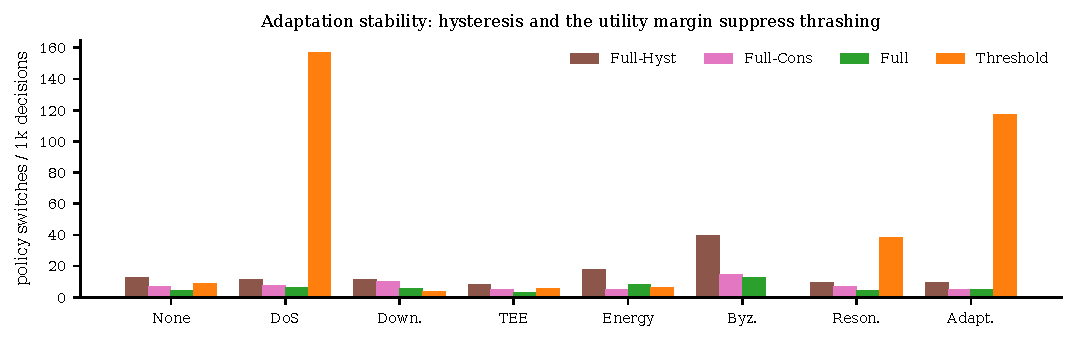
\includegraphics[width=\linewidth]{figures/fig_switching.pdf}
\caption{Policy switches per $1{,}000$ decisions by scenario. Hysteresis and the
utility margin reduce switching by more than half relative to the same controller
without them, including under the adaptive and Byzantine scenarios.}
\label{fig:switching}
\end{figure}

% Generated by make_paper_assets.py — do not edit by hand; regenerate.
\begin{table*}[t]
\centering
\scriptsize
\setlength{\tabcolsep}{3.5pt}
\caption{Policy switches per 1,000 decisions (mean over 10 seeds). A switch is a
change of security level for the same operation class between epochs; the final
column averages the seven attack scenarios. Lower is better; static policies are
omitted because they never switch.}
\label{tab:switching}
\begin{tabular}{lccccccccc}
\toprule
Policy & None & DoS & Down. & TEE & Energy & Byz. & Reson. & Adapt. & Mean \\
\midrule
Threshold & 8.6 & 157.2 & 3.8 & 5.6 & 6.3 & 0.7 & 38.6 & 117.2 & 47.1 \\
Risk-Only & 18.7 & 12.5 & 11.9 & 11.6 & 20.3 & 25.8 & 9.6 & 9.1 & 14.4 \\
Inv.-Only & 0.6 & 6.5 & 0.4 & 0.5 & 0.8 & 0.2 & 4.4 & 0.5 & 1.9 \\
Full$-$Hyst & 12.5 & 11.6 & 11.3 & 8.3 & 18.1 & 39.5 & 9.2 & 9.3 & 15.3 \\
Full$-$Cons & 6.9 & 7.7 & 9.9 & 4.8 & 4.9 & 14.7 & 6.7 & 4.9 & 7.7 \\
\textbf{Full} & 4.3 & 6.1 & 5.9 & 3.4 & 8.2 & 12.5 & 4.5 & 4.8 & 6.5 \\
\emph{Oracle} & 4.1 & 6.4 & 5.6 & 6.1 & 0.0 & 3.1 & 3.2 & 3.2 & 3.9 \\
\bottomrule
\end{tabular}
\end{table*}


\paragraph{Systems cost.} Full's median decision latency is $2.27$\,ms and its
$99$th percentile is $5.54$\,ms, with $0.288$\,mJ per granted decision,
$14$\,KB SRAM and $86$\,KB flash. Static-High is $6.00$\,ms and $0.728$\,mJ with
$4$\,KB and $28$\,KB; Threshold is $1.33$\,ms and $0.295$\,mJ; Invariant-Only is
$1.34$\,ms and $0.239$\,mJ. The full controller is therefore cheaper than a
static-high posture in latency (by a factor of $2.6$) and energy (by a factor of
$2.5$), because it selects the cheapest admissible action most of the time and
pays for deep inspection only when the belief or I3 requires it. It is more
expensive than Invariant-Only by $0.049$\,mJ and $28$\,KB of flash, which is the
cost of the belief filter and trust weights.

These are analytical model outputs, not silicon measurements. The per-layer
constants come from datasheet-level operation counts and the tier mix of
\cref{sec:system-model}; the reported p50/p99 are therefore best read as
relative comparisons between postures, not as predictions for a specific board.
The footprint numbers are model estimates for the static image of the decision
layer and exclude the cryptographic library, which would be shared with any
baseline. A deployment would replace the cost model with a measured profile; the
controller only consumes the resulting scalar costs, so the decision logic does
not change.

% Generated by make_paper_assets.py — do not edit by hand; regenerate.
\begin{table}[t]
\centering
\small
\caption{Systems cost per granted decision, averaged over all 70 runs.
Latency and energy are \emph{analytical model} outputs from datasheet-level
operation costs and the tier mix; SRAM/flash are model footprints, not
silicon measurements.}
\label{tab:systems}
\begin{tabular}{lccccc}
\toprule
Policy & p50 (ms) & p99 (ms) & Energy (mJ) & SRAM (KB) & Flash (KB) \\
\midrule
Static-High & 6.00 & 6.00 & 0.728 & 4.0 & 28.0 \\
Static-Med & 3.40 & 4.70 & 0.472 & 14.0 & 86.0 \\
Static-Low & 0.90 & 0.90 & 0.047 & 4.0 & 28.0 \\
Threshold & 1.33 & 5.17 & 0.295 & 6.0 & 34.0 \\
Risk-Only & 0.90 & 4.74 & 0.113 & 12.0 & 74.0 \\
Inv.-Only & 1.34 & 5.00 & 0.239 & 9.0 & 58.0 \\
Full$-$Hyst & 1.51 & 5.54 & 0.243 & 14.0 & 86.0 \\
Full$-$Cons & 2.40 & 5.60 & 0.294 & 12.0 & 74.0 \\
\textbf{Full} & 2.27 & 5.54 & 0.288 & 14.0 & 86.0 \\
\emph{Oracle} & 2.23 & 5.59 & 0.281 & 14.0 & 86.0 \\
\bottomrule
\end{tabular}
\end{table}


\paragraph{Ablation.} \Cref{tab:ablation} summarises the component analysis over
the seven attack scenarios. Full has the lowest malicious-grant rate ($0.177$) of
the four ablated variants and utility within $0.001$ of Full$-$Hyst; among all
policies that enforce the floor, only Static-High and Oracle have lower exposure
($0.127$ and $0.148$), at lower utility and as an oracle upper bound,
respectively. Removing hysteresis raises malicious grants to $0.209$ and
switches to $15.3$; removing consistency weighting raises malicious grants to
$0.184$ and the energy-scenario Brier score to $0.455$; removing the belief
entirely (Invariant-Only) gives $0.312$ and Brier $0.296$. The order is consistent: the invariant layer carries
safety, the belief and trust weighting carry detection, and hysteresis carries
stability. No single component is responsible for all three.

% Generated by make_paper_assets.py — do not edit by hand; regenerate.
\begin{table}[t]
\centering
\small
\caption{Component ablation (Full policy), means over the seven attack scenarios.
Brier$_{\text{energy}}$ isolates the attack-inflation scenario, where uniform
modality fusion is misled. Switches are per 1,000 decisions.}
\label{tab:ablation}
\resizebox{\textwidth}{!}{%
\begin{tabular}{lcccccc}
\toprule
Variant & IVR/1k & Malicious grant & Utility & Brier$_{\text{energy}}$ & Switches/1k & Energy (mJ) \\
\midrule
Inv.-Only & 0.00 & 0.312 & 0.102 & 0.296 & 1.9 & 0.239 \\
Full$-$Hyst & 0.00 & 0.209 & 0.119 & 0.003 & 15.3 & 0.243 \\
Full$-$Cons & 0.00 & 0.184 & 0.118 & 0.455 & 7.7 & 0.294 \\
\textbf{Full} & 0.00 & 0.177 & 0.120 & 0.003 & 6.5 & 0.288 \\
\emph{Oracle} & 0.00 & 0.148 & 0.128 & 0.000 & 3.9 & 0.281 \\
\bottomrule
\end{tabular}}
\end{table}


\subsection{Sensitivity of the actuation floor}
\label{sec:rq5-floor}

The guarantee in RQ1 is only as strong as the floor it enforces, so we repeat
the Full experiment with four I1 variants: mutual authentication with header
inspection (the default), attestation with header inspection, mutual
authentication with deep inspection, and attestation with deep inspection.
\Cref{tab:floor} reports the result. Every variant keeps IVR at zero, which is
the expected consequence of enforcing the floor; the differences are in residual
exposure, utility and energy. Strengthening I1 from mutual authentication with
header inspection to attestation with deep inspection reduces malicious grants
from $0.177$ to $0.165$ (about $7\,\%$), lowers attack-scenario utility only
from $0.120$ to $0.115$, and raises modelled energy from $0.279$ to
$0.363$\,mJ (about $30\,\%$). Every variant keeps IVR at zero. The two
intermediate floors are not strictly ordered---attestation with header inspection
gives $0.170$ and mutual authentication with deep inspection gives $0.171$---which
is within seed noise and illustrates that the components buy different, partly
substitutable evidence rather than a single strength scale.

This sensitivity is the practical answer to the \texttt{tee} result. Since the
belief cannot be trusted when the anchor is subverted, the defensible response is
to choose the floor using an explicit risk budget rather than to tune the
estimator until it looks better on the out-of-model scenario. \Cref{tab:floor}
makes that choice legible.

% Generated by floor_sensitivity.py — do not edit by hand; regenerate.
\begin{table}[t]
\centering
\caption{Sensitivity to the actuation floor (I1), Full policy, 10 seeds.
IVR, false denial and energy are means over all eight scenarios; malicious
grant and utility (marked $^{\ast}$) are means over the seven attack scenarios.
Every floor keeps invariant violations at zero; a stronger floor buys lower
residual exposure at a utility and energy cost.}
\label{tab:floor}
\resizebox{\textwidth}{!}{%
\begin{tabular}{lccccc}
\toprule
Actuation floor & IVR/1k & Malicious grant$^{\ast}$ & Utility$^{\ast}$ & False deny & Energy (mJ) \\
\midrule
mutual auth + header IDS & 0.00 & 0.177 & 0.120 & 0.026 & 0.279 \\
attestation + header IDS & 0.00 & 0.170 & 0.118 & 0.028 & 0.288 \\
mutual auth + deep IDS & 0.00 & 0.171 & 0.117 & 0.029 & 0.357 \\
attestation + deep IDS & 0.00 & 0.165 & 0.115 & 0.030 & 0.363 \\
\bottomrule
\end{tabular}}
\end{table}


\subsection{Trace-derived calibration}
\label{sec:trace}

The simulator's network-intensity prior is calibrated against the public IoT-23
capture \cite{garcia2020iot}. We extract individual \texttt{conn.log.labeled}
captures, aggregate packet counts into $60$\,s bins, separate benign from
malicious bins using the capture labels, and fit a log-normal rate model. The
contrast is the difference of mean log rates, estimated only within captures that
contain both labels so that a device/context difference between captures cannot
masquerade as an attack effect. The fitted benign mean log-rate is $-3.103$ and
the malicious mean is $-1.413$, giving a contrast of $1.689$ with a
$2{,}000$-sample stratified bin bootstrap interval of $[1.652,1.726]$
(\cref{tab:trace}). The two within-capture estimates are $1.131$ and $2.570$;
that spread, not the bin-level interval, is the honest between-capture
uncertainty, and the bin bootstrap understates it because consecutive bins are
autocorrelated. The simulator uses a benign mean of $4.20$ and a DoS mean of
$5.889$, a contrast of $1.689$. The absolute rates differ because a sparse
honeypot capture is not comparable to per-node application telemetry, so only the
contrast is matched. The dispersion is not matched either: the simulator's
network standard deviation is $0.50$ benign and $0.55$ under DoS, against pooled
log-rate standard deviations of $0.65$ and $0.86$ in the trace, so no
distributional-shape claim is made.

\Cref{fig:belief-trace} shows the belief, the minimum modality trust and the
consistency score on one adaptive-attack run. The belief rises inside the attack
windows and decays after them; the trust on the network modality falls when the
spoofed context diverges from the device anchor and recovers slowly; the
consistency score leads the belief during the early part of an attack. The
figure is a single seed and is included as an illustration of the mechanism, not
as evidence of average performance; the aggregate numbers are in
\cref{tab:calibration,tab:detection}.

\begin{figure}[t]
\centering
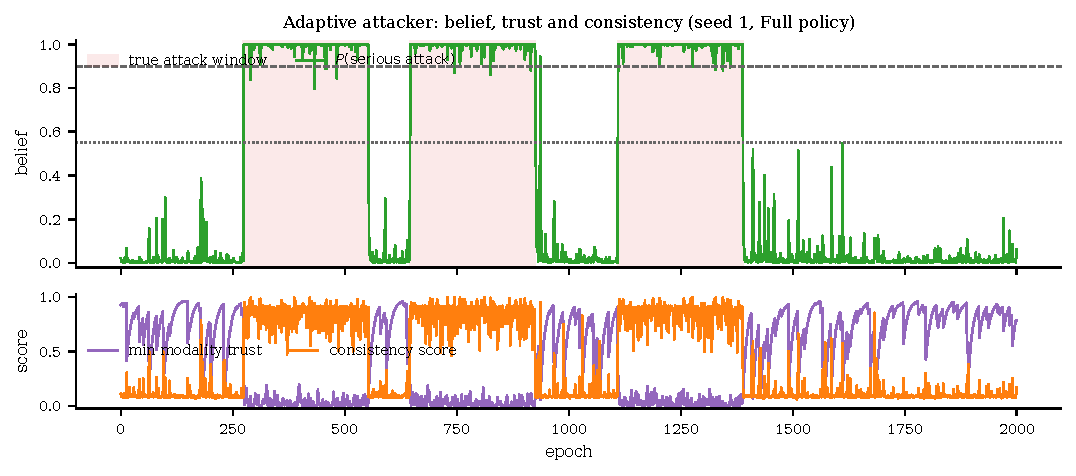
\includegraphics[width=\linewidth]{figures/fig_belief_trace.pdf}
\caption{Belief, minimum modality trust and consistency score on one adaptive
attack run (seed 1, Full policy). The belief rises in the attack windows and
decays afterwards; distrust is fast and restoration is slow. Single-seed
illustration, not an aggregate result.}
\label{fig:belief-trace}
\end{figure}

\begin{figure}[t]
\centering
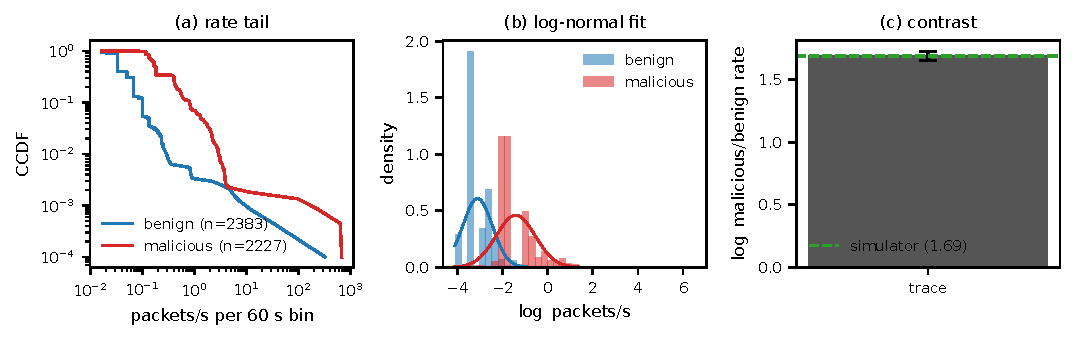
\includegraphics[width=\linewidth]{figures/fig_trace_calibration.pdf}
\caption{IoT-23 calibration of the network-intensity prior. Benign and malicious
$60$\,s bins are separated by capture label; the fitted mean-log-rate contrast is
$1.689$ with per-capture values $1.131$ and $2.570$. The simulator matches the
contrast, not the absolute rate or the dispersion.}
\label{fig:trace}
\end{figure}

% Generated by make_paper_assets.py from trace_priors.json.
\begin{table}[t]
\centering
\small
\caption{IoT-23 trace calibration of the network-intensity prior. The contrast is
the difference of mean $\log$ rates over 60\,s bins, estimated only within
captures that contain both benign and malicious traffic. The bracket is a
2{,}000-sample stratified bin bootstrap, which treats bins as independent; the
per-capture values show the between-capture spread. Absolute rates are not
comparable to per-node simulator telemetry; only the contrast is calibrated.}
\label{tab:trace}
\begin{tabular}{lcc}
\toprule
Quantity & Trace & Simulator \\
\midrule
Benign 60\,s bins & 2383 & -- \\
Malicious 60\,s bins & 2227 & -- \\
Benign $\log$ rate (mean) & -3.103 & 4.20 \\
Malicious $\log$ rate (mean) & -1.413 & 5.89 \\
Log-rate contrast & 1.689 [1.652, 1.726] & 1.689 \\
\quad per-capture contrast & 1.131, 2.570 & -- \\
\bottomrule
\end{tabular}
\end{table}


\subsection{Summary of the evidence}
\label{sec:eval-summary}

The five research questions receive the following answers. RQ1: yes, with a
zero IVR in every scenario, and the zero is structural rather than a property of
the estimator (\cref{tab:ivr,tab:ivr-byop}). RQ2: the guarantee costs little
utility relative to Static-High ($+0.036$) and gains more against Threshold
($+0.043$), it cuts false denials by a factor of three, but it grants more
malicious requests than Static-High ($0.177$ versus $0.127$), mostly in the
out-of-model TEE scenario, because the invariant floor bounds the action, not the
adversary's credential (\cref{tab:utility,tab:falsedeny,tab:exposure}). RQ3: the
belief is well calibrated under DoS, in-model downgrade, energy inflation,
resonant, Byzantine and adaptive attacks, and fails only when the attestation
anchor is subverted; trust weighting is worth a factor of about $140$ in Brier score
under energy inflation (\cref{tab:calibration,tab:detection}). RQ4: the
per-operation envelope denies $0.029$ of safety requests against $0.088$ for
Static-High, and every residual denial is a mechanism false positive, not a
policy choice (\cref{tab:safety}). RQ5: switching is $6.5$ per $1{,}000$
decisions against $15.3$ without hysteresis, and the full controller is cheaper
than Static-High in latency ($2.27$ versus $6.00$\,ms) and energy ($0.288$ versus
$0.728$\,mJ) at the cost of $28$\,KB of flash relative to Invariant-Only
(\cref{tab:switching,tab:systems}). Strengthening the actuation floor reduces
exposure without changing IVR (\cref{tab:floor}). The next section discusses what
these results do and do not establish.
